\chapter{Mapeamento Sistemático}
Este capítulo abordará o processo de Mapeamento Sistemático adotado neste estudo, com o objetivo de levantar métodos, técnicas e padrões utilizados na implementação de acessibilidade em aplicações \emph{mobile}.


\section{Protocolo de Mapeamento Sistemático}
O termo Mapeamento Sistemático da Literatura (MSL) se refere a uma revisão ampla de estudos primários existentes em um tema específico e visa identificar as evidências disponíveis nessa área \cite{Kitchenham2007}.
O método de Mapeamento Sistemático adotado foi o de Kitchenham, descrito em \citeonline{Silva2009}.
De acordo com o método, foi desenvolvido um protocolo de revisão com intuito de responder as seguintes questões:
\begin{enumerate}
\item Quais são as principais técnicas, padrões e métodos utilizados no desenvolvimento de aplicações móveis acessíveis para deficientes visuais?
\item Quais são as tecnologias utilizadas no desenvolvimento dessas soluções?
\item Para quais plataformas as soluções foram propostas?
\item Quais são os públicos alvos dessas soluções?
\end{enumerate}

O \emph{Parfisal}\footnote{\url{https://parsif.al/}}, ferramenta \emph{online} que auxilia no desenvolvimento de Revisões Sistemáticas da Literatura, foi utilizado neste estudo.
Com ele foi possível importar os resultados das buscas nas bases, identificar os artigos duplicados, definir os critérios para inclusão e exclusão, realizar a seleção dos estudos e, por fim, obter os relatórios para construção dos artefatos que apresentam o processo e os resultados desse MSL.

\subsection{Bases de Dados}
Cinco bases de dados científicos foram escolhidas neste trabalho, a \emph{IEEE Xplore}\footnote{\url{https://ieeexplore.ieee.org}}, onde estão disponíveis conteúdos técnicos e científicos publicados pelo \emph{Institute of Electrical and Electronics Engineers (IEEE)} e seus parceiros,
a \emph{Scopus}\footnote{\url{https://www.scopus.com}}, que é mantida pela \emph{Elsevier} e combina um abrangente banco de dados de resumos e citações de literatura acadêmica em diversas áreas, a \emph{ScienceDirect}\footnote{\url{https://www.sciencedirect.com}}, principal plataforma da \emph{Elsevier} de literatura revisada por pares,
a \emph{ACM Digital Library}\footnote{\url{https://dl.acm.org}}, uma plataforma de pesquisa que conta com textos completos de todas as publicações da \emph{Association for Computing Machinery (ACM)} e de uma curada coleção de publicações de editoras selecionadas e a \emph{PubMed}\footnote{\url{https://pubmed.ncbi.nlm.nih.gov}},
plataforma gratuita que conta com uma base de dados com mais de 33 milhões de citações e resumos da literatura biomédica.

\subsection{\emph{String} de Busca}
Para realização da busca dos artigos, um conjunto de palavras-chave e sinônimos foi definido de acordo com o tema deste trabalho, como é mostrado no \autoref{qua-pal-sin}.

\begin{quadro}[htb]
\caption{\label{qua-pal-sin}Palavras-chave e Sinônimos.}
\begin{tabular}{|c|c|}
  %\hline
    \hline
   \textbf{Palavra-chave} & \textbf{Sinônimos (Inglês)} \\ \hline
    Acessibilidade & \emph{Accessibility} \\ \hline
    Aplicativo & \emph{Application, App} \\ \hline
    Deficiência visual & \emph{Visual impairment, Visually impaired} \\ \hline
    Móvel & \emph{Mobile, Smartphone} \\ \hline
   % \hline
\end{tabular}
\legend{Fonte: Autor}
\end{quadro}

Com o objetivo de manter a consistência da busca nas diferentes bases, foi gerada, a partir das palavras-chave, a \emph{string} de busca genérica indicada no \autoref{qua-str-gen}.
As palavras-chave que possuem sinônimos aparecem na \emph{string} entre parêntesis com o operador \emph{OR}, visando incluir os resultados que contenham um dos termos, para indicar que esses termos são sinônimos no contexto do tema abordado neste trabalho.

\begin{quadro}[htb]
\caption{\label{qua-str-gen}\emph{String} genérica.}
\begin{tabular}{|m{11.5cm}|}
  %\hline
    \hline
    \textbf{\emph{String} genérica} \\
    \hline
    \emph{accessibility AND (“visual impairment” OR “visually impaired”) AND (mobile OR smartphone) AND (app OR application)} \\ \hline
   % \hline
\end{tabular}
\legend{Fonte: Autor}
\end{quadro}

A \emph{string} genérica serviu de modelo para criação das \emph{strings} específicas, indicadas no \autoref{qua-str-esp}, de acordo com as particularidades de cada base de busca.
As \emph{strings} específicas buscam pelas palavras-chave nos títulos e resumos dos artigos, afim de encontrar os que focam no tema proposto neste estudo, não considerando os que apenas citam as palavras-chave ao longo texto.

\begin{quadro}[htb]
\caption{\label{qua-str-esp}\emph{Strings} específicas para busca em cada base.}
\begin{tabular}{|m{3.5cm} | m{11.5cm}|}
   \hline
   \textbf{Base} & \textbf{\emph{String} de busca} \\ \hline
    \emph{ACM Digital Library} & \emph{(Abstract:(accessibility) OR Title:(accessibility)) AND (Abstract:("visual impairment" OR "visually impaired") OR Title:("visual impairment" OR "visually impaired")) AND (Abstract:(smartphone OR mobile) OR Title:(smartphone OR mobile)) AND (Abstract:(app OR application) OR Title:(app OR application))} \\ \hline
    \emph{IEEE Xplore} & \emph{(("Abstract":accessibility OR "Document Title":accessibility) AND ("Document Title":mobile OR "Document Title":smartphone OR "Abstract":mobile OR "Abstract":smartphone) AND ("Document Title":"visual impairment" OR "Abstract":"visual impairment" OR "Document Title":"visually impaired" OR "Abstract":"visually impaired") AND ("Document Title":app OR "Document Title":application OR "Abstract":app OR "Abstract":application))} \\ \hline
    \emph{PubMed} & \emph{(accessibility[Abstract] OR accessibility[Title]) AND ("visually impaired"[Abstract] OR "visual impairment"[Abstract] OR "visually impaired"[Title] OR "visual impairment"[Title]) AND (mobile[Abstract] OR smartphone[Abstract] OR mobile[Title] OR smartphone[Title]) AND (app[Title] OR app[Abstract] OR application[Title] OR application[Abstract])} \\ \hline
    \emph{ScienceDirect} & \emph{Title, abstract, keywords: accessibility AND ("visual impairment" OR "visually impaired") AND (mobile OR smartphone) AND (app OR application)} \\ \hline
    \emph{Scopus} & \emph{TITLE-ABS (accessibility AND ("visual impairment" OR "visually impaired") AND (smartphone OR mobile) AND (app OR application))} \\ \hline
\end{tabular}
\legend{Fonte: Autor}
\end{quadro}

A busca nas bases de dados selecionadas foi realizada no dia 04 de outubro de 2021 e retornou um total de 258 resultados.
Como mostra a \autoref{fig_art_enc}, a maior quantidade de resultados foi encontrada na \emph{Scopus}, isso acontece porque ela possui, de acordo com seu site\footnote{\url{https://www.elsevier.com/pt-br/solutions/scopus}}, o maior banco de dados de resumos e citações da literatura com revisão por pares.
Em seguida aparecem a \emph{ACM Digital Library} e a \emph{IEEE Xplore} cujas principais publicações são na área de computação, e elétrica no caso da IEEE\@.
Por fim, com as menores quantidades, a \emph{ScienceDirect}, com publicações nas mais diversas áreas da ciência e a \emph{PubMed} com publicações na área biomédica, justificando os menores resultados, visto que a busca foi realizada visando encontrar técnicas, métodos e padrões para o desenvolvimento de aplicações móveis acessíveis.

\begin{figure}[htb]
	\caption{\label{fig_art_enc}Quantidade de artigos encontrados por base.}
	\begin{center}
	    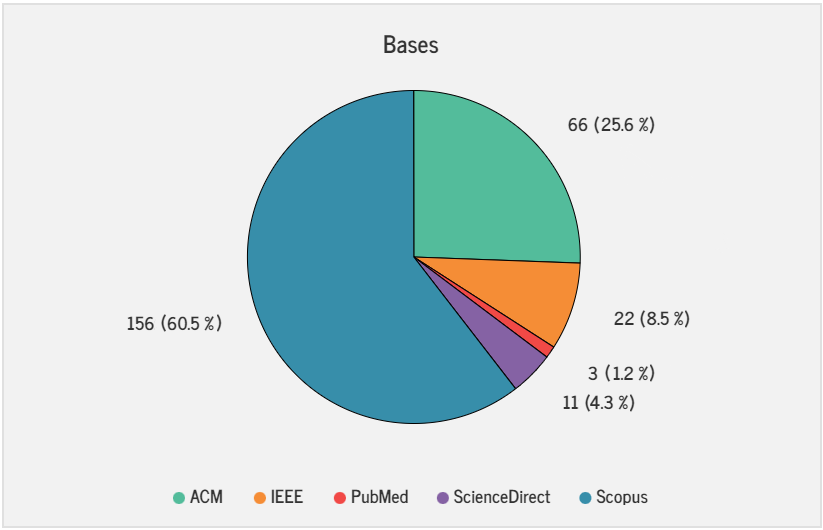
\includegraphics[scale=0.7]{Imagens/msl/artigos_encontrados.png}
	\end{center}
	\legend{Fonte: Autor}
\end{figure}

\subsection{Critérios de Inclusão e Exclusão}

Critérios de inclusão e exclusão foram definidos visando a coerência dos artigos selecionados com o tema deste trabalho, bem como a remoção de artigos incompletos ou indisponíveis.
Os critérios são:

\textbf{Critérios de Inclusão}
\begin{itemize}
  \item O artigo deve propor método, técnica ou padrão para o desenvolvimento de aplicações móveis com acessibilidade para deficientes visuais;
  \item O artigo deve estar disponível na \emph{web};
  \item O artigo deve apresentar texto completo em formato eletrônico;
  \item O artigo deve estar escrito em português ou inglês.
\end{itemize}

\textbf{Critérios de Exclusão}
\begin{itemize}
  \item O artigo não apresenta proposta de aplicação móvel como solução;
  \item O artigo não apresenta aplicativo desenvolvido no contexto do tema deste trabalho;
  \item O artigo é um livro ou parte de um;
  \item O artigo foi publicado antes de 2016;
  \item O artigo está incompleto, indisponível ou duplicado.
\end{itemize}

No processo de seleção dos estudos, inicialmente, foi aplicado o critério de exclusão de artigos duplicados e, em seguida, o de artigos publicados antes de 2016, rejeitando 48 e 65 artigos, respectivamente.
Esses critérios foram priorizados por não haver a necessidade da leitura dos títulos e resumos dos artigos para serem aplicados.
Por fim, após a leitura dos títulos e resumos, mais 112 artigos foram rejeitados, totalizando 225 artigos.
Assim, sendo aceitos 33 artigos para leitura completa e análise.
A \autoref{fig_res_sel} apresenta o resultado dessa seleção.

\begin{figure}[htb]
	\caption{\label{fig_res_sel}Quantidade de artigos aceitos, rejeitados e duplicados na seleção.}
	\begin{center}
	    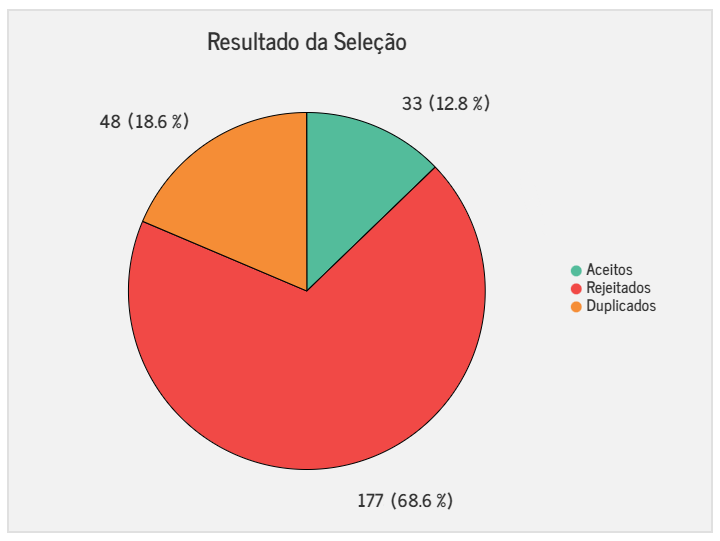
\includegraphics[scale=0.7]{Imagens/msl/resultado_selecao.png}
	\end{center}
	\legend{Fonte: Autor}
\end{figure}

A \autoref{fig_res_sel_base} mostra o resultado da seleção para cada base de busca.
Não houve priorização de bases ao rejeitar artigos duplicados, visto que a ferramenta utilizada possui uma funcionalidade que indica esses artigos, sendo necessário apenas a confirmação.
Com isso, algumas bases como a \emph{PubMed}, cujo resultado da busca retornou apenas 3 artigos sendo 1 duplicado, acabou apresentando poucos ou nenhum artigo aceito.

\begin{figure}[htb]
	\caption{\label{fig_res_sel_base}Quantidade de artigos aceitos e rejeitados por base.}
	\begin{center}
	    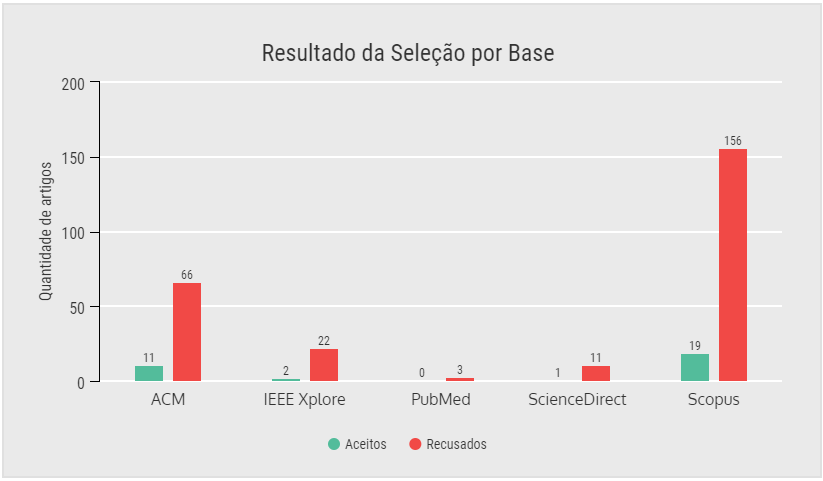
\includegraphics[scale=0.6]{Imagens/msl/resultado_selecao_base.png}
	\end{center}
	\legend{Fonte: Autor}
\end{figure}

\newpage

A frequência dos artigos rejeitados, de acordo com os critérios de exclusão, sendo que, para rejeição, o artigo deveria atender a pelo menos um desses critérios, pode ser observada no gráfico da \autoref{fig_art_rej}, onde é listada para cada critério.

\begin{figure}[htb]
	\caption{\label{fig_art_rej}Quantidade de artigos rejeitados por critério de exclusão.}
	\begin{center}
	    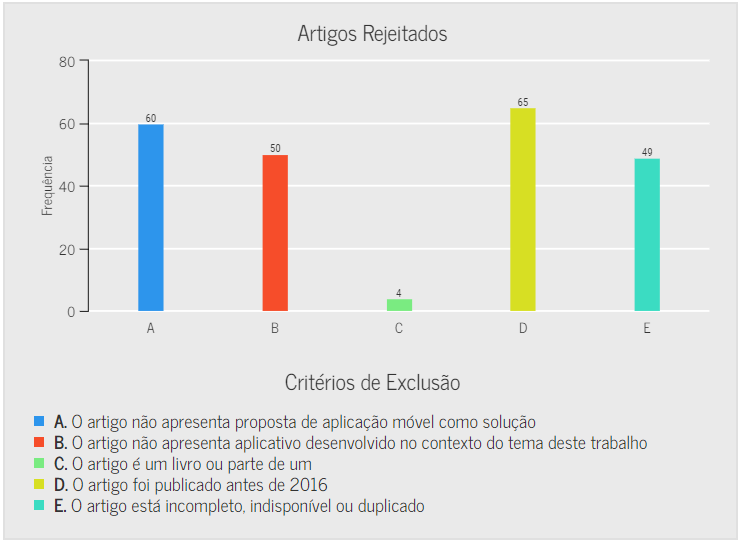
\includegraphics[scale=0.6]{Imagens/msl/artigos_rejeitados.png}
	\end{center}
	\legend{Fonte: Autor}
\end{figure}

Os critérios de exclusão levaram em consideração, principalmente, aspectos como divergência com o tema deste trabalho e não apresentação de aplicação desenvolvida para dispositivos móveis.
Os critérios D e E aparecem com grande frequência na \autoref{fig_art_rej}, valendo ressaltar a ordem na avaliação dos critérios (E, D, A, B e C), onde os artigos que se enquadraram em um dos critérios foram rejeitados, não sendo considerados para avaliação nos demais.
É comum que o critério D seja utilizado no próprio processo de busca dos artigos, filtrando apenas os anos de interesse, porém, como não foi possível adicionar esse filtro às \emph{strings} de busca para todas as bases, foi optado por não utiliza-lo, para manter a consistência nos resultados das buscas.

Após a aplicação dos critérios de exclusão, através da leitura e análise dos títulos e resumos, os artigos restantes, a priori, mostraram se enquadrar em todos os critérios de inclusão.
Assim, a \autoref{fig_art_act_ano} exibe a distribuição desses artigos por ano de publicação e base de busca, mostrando uma clara tendência de alta anual, nos últimos 5 anos, na quantidade de artigos que abordam o tema deste trabalho.
A base \emph{PubMed} foi desconsiderada nessa figura, visto que nenhum artigo dela foi selecionado como mostrou a \autoref{fig_art_rej}.


\begin{figure}[htb]
	\caption{\label{fig_art_act_ano}Quantidade de artigos aceitos por ano e base.}
	\begin{center}
	    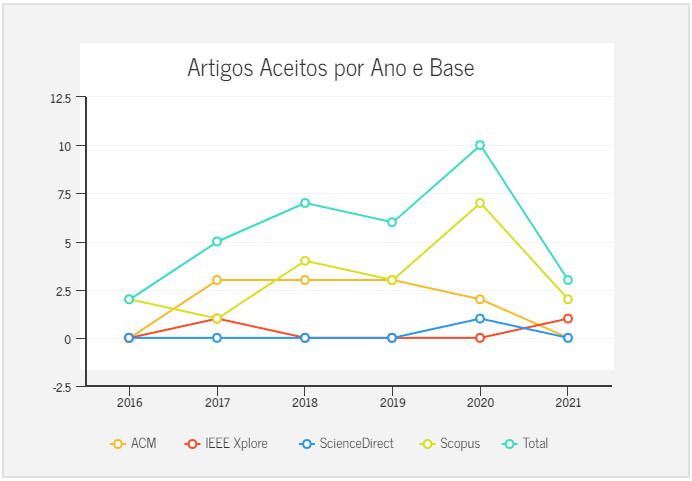
\includegraphics[scale=0.85]{Imagens/msl/artigos_aceitos_ano_base.png}
	\end{center}
	\legend{Fonte: Autor}
\end{figure}

\newpage{}

\subsection{Fase de Extração}

Durante a fase de extração, uma análise mais aprofundada dos artigos foi realizada, inicialmente com intuito de reaplicar os critérios já definidos e utilizados na fase anterior.
O resultado dessa última filtragem pode ser visto na \autoref{fig_fas_ext}.

\begin{figure}[htb]
	\caption{\label{fig_fas_ext}Artigos aceitos e rejeitados na fase de extração.}
	\begin{center}
	    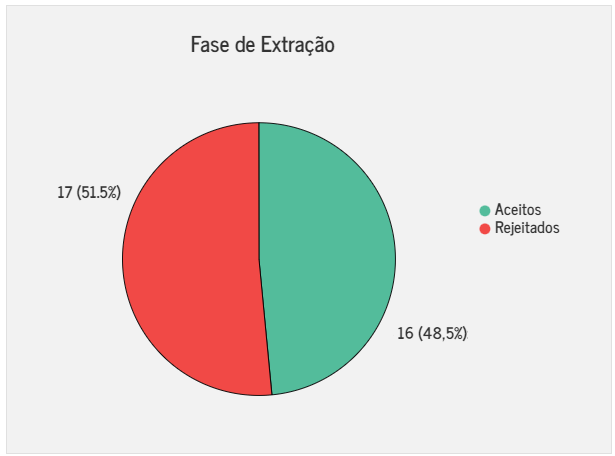
\includegraphics[scale=0.85]{Imagens/msl/fase_extracao_artigos.png}
	\end{center}
	\legend{Fonte: Autor}
\end{figure}

Como a aplicação inicial dos critérios foi realizada com base apenas na leitura dos títulos e resumos dos estudos, não foi possível garantir que os artigos aceitos realmente não se enquadravam nos critérios de exclusão.
Assim, com a análise mais aprofundada e leitura completa dos textos, foi possível identificar 18 artigos que se enquadravam em algum desses critérios, como mostrou a \autoref{fig_fas_ext}.

\newpage

A \autoref{fig_art_rej_fas_ext} mostra a frequência de artigos que foram rejeitados por cada critério de exclusão.
Apenas os critérios com frequência maior que 0 foram considerados na figura.
O principal motivo para rejeição foi o B, onde os trabalhos apresentavam aplicações móveis que não haviam sido desenvolvidas com foco na acessibilidade da aplicação em si.
O segundo foi o A, onde os estudos não apresentavam uma aplicação móvel com acessibilidade à PDV como solução.

\begin{figure}[htb]
	\caption{\label{fig_art_rej_fas_ext}Artigos rejeitados na fase de extração por critério exclusão.}
	\begin{center}
	    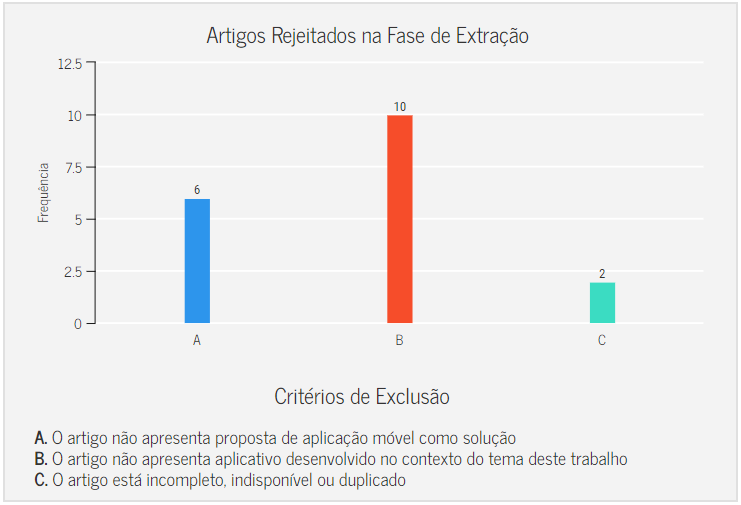
\includegraphics[scale=0.7]{Imagens/msl/artigos_rejeitados_fase_extracao.png}
	\end{center}
	\legend{Fonte: Autor}
\end{figure}

Os 15 estudos aceitos na fase de extração foram reunidos no \autoref{qua-art-ext} com a listagem de informações como o título do estudo, referência e o nome da base de dados em que o artigo foi encontrado.

\begin{quadro}[htb!]
\caption{\label{qua-art-ext}Artigos aceitos na fase de extração.}
\begin{tabular}{|m{1.0cm} | m{8.1cm} | m{2.6cm} | m{2.5cm}|}
  %\hline
    \hline
    \textbf{Sigla} &\textbf{Título} & \textbf{Referência} & \textbf{Base de dados} \\ \hline
    AM1 & \emph{A Mobile Educational Game Accessible to All, Including Screen Reading Users on a Touch-Screen Device} & \cite{Leporini2017} & \emph{ACM Digital Library} \\ \hline
    AM2 & \emph{A model-driven approach to cross-platform development of accessible business apps} & \cite{Christoph2020} & \emph{ACM Digital Library} \\ \hline
    AM3 & \emph{An Accessible Roller Coaster Simulator for Touchscreen Devices: An Educational Game for the Visually Impaired} & \cite{Biase2018} & \emph{IEEE Xplore} \\ \hline
    AM4 & \emph{Application for the Configuration and Adaptation of the Android Operating System for the Visually Impaired} & \cite{Oliveira2018} & \emph{ACM Digital Library} \\ \hline
    AM5 & \emph{Blind and visually impaired user interface to solve accessibility problems} & \cite{Shera2021285} & \emph{Scopus} \\ \hline
    AM6 & \emph{Design and development of a mobile app of drug information for people with visual impairment} & \cite{Amariles2020} & \emph{ScienceDirect} \\ \hline
    AM7 & \emph{Designing multimodal mobile interaction for a text messaging application for visually impaired users} & \cite{Duarte2017} & \emph{Scopus} \\ \hline
    AM8 & \emph{Do You like My Outfit? Cromnia, a Mobile Assistant for Blind Users} & \cite{Giuliana2018} & \emph{ACM Digital Library} \\ \hline
    AM9 & \emph{Improved and Accessible E-Book Reader Application for Visually Impaired People} & \cite{Heesook2017} & \emph{ACM Digital Library} \\ \hline
    AM10 & \emph{MathMelodies 2: A Mobile Assistive Application for People with Visual Impairments Developed with React Native} & \cite{Ducci2018} & \emph{ACM Digital Library} \\ \hline
    AM11 & \emph{Object Recognition and Hearing Assistive Technology Mobile Application Using Convolutional Neural Network} & \cite{Caballero2020} & \emph{ACM Digital Library} \\ \hline
    AM12 & \emph{QUIMIVOX MOBILE 2.0: Application for Helping Visually Impaired People in Learning Periodic Table and Electron Configuration} & \cite{Oliveira2019} & \emph{ACM Digital Library} \\ \hline
    AM13 & \emph{``Talkin' about the weather'': Incorporating TalkBack functionality and sonifications for accessible app design} & \cite{Tomlinson2016377} & \emph{Scopus} \\ \hline
    AM14 & \emph{Users’ perception on usability aspects of a braille learning mobile application ‘mBRAILLE’} & \cite{Nahar2019100} & \emph{Scopus} \\ \hline
    AM15 & \emph{WordMelodies: Supporting Children with Visual Impairment in Learning Literacy} & \cite{Mascetti2019} & \emph{ACM Digital Library} \\ \hline
   % \hline
\end{tabular}
\legend{Fonte: Autor}
\end{quadro}